\section{Results}\label{sec:results}
%Results
%Show effect of colorspaces, blur, annealed mean
%Compare results of architecture (images, error plot, feature maps)

In section \ref{sec:method} all the different techniques and methods used resulted in multiple experiments. This sections shows the different results of each experiment, setting the foundation for the discussion in section \ref{sec:discussion}.

\subsection{Colorspace}
To asses the effect of different colorspaces, a comparison is made between CIELab and YCbCr. The compact network is trained on the landscape set for both the YCbCr and CIELab color space, for a total of 20 epochs. The result is shown in figure \ref{fig:YCbCr_vs_CIELab}.

\begin{figure}[h!]
	\centering
	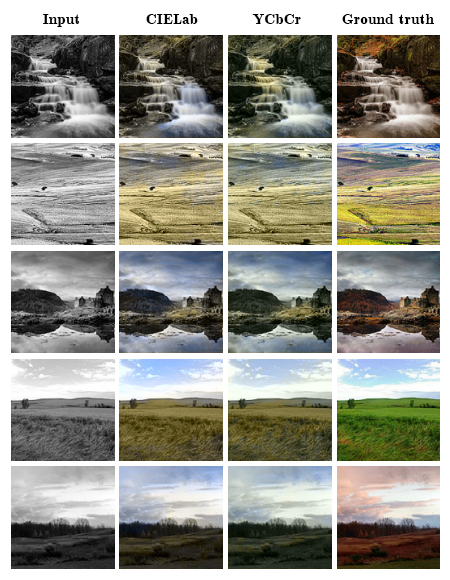
\includegraphics[width=0.6\textwidth]{YCbCr_vs_CIELab}
	\caption{YCbCr vs CIELab}
	\label{fig:YCbCr_vs_CIELab}
\end{figure}

\subsection{Gaussian blur}
The comparison between different Gaussian blur kernel standard deviations is seen in figure \ref{fig:blur}. The comparison was done with the compact network, trained on the landscape dataset. Note that the standard deviation only comes into play during training, since the target output layer is blurred the target less noisy. 

\begin{figure}[h]
	\centering
	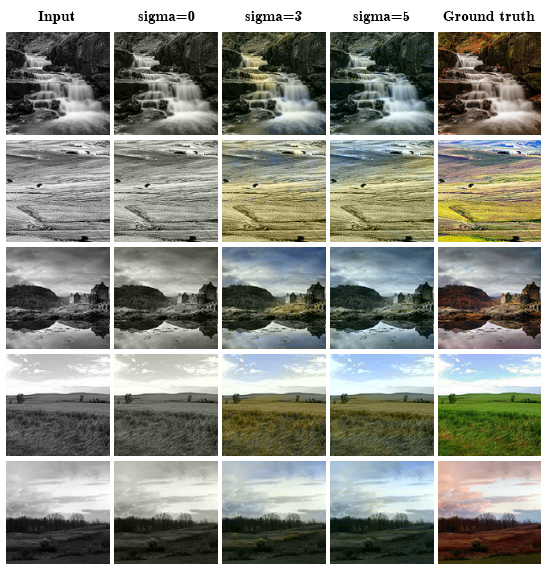
\includegraphics[width=0.6\textwidth]{blur}
	\caption{Blur}
	\label{fig:blur}
\end{figure}

\subsection{Network output}
In this section the colorization result of the different networks are shown, by propagating an image through the trained networks. These results are shown in figure \ref{fig:results}. Note that the annealed mean temperature is set to $0.4$. The optimal setting for the temperature can vary for each network, however keeping this into account sound conclusions can still be made. 
\begin{figure}[h]
	\centering
	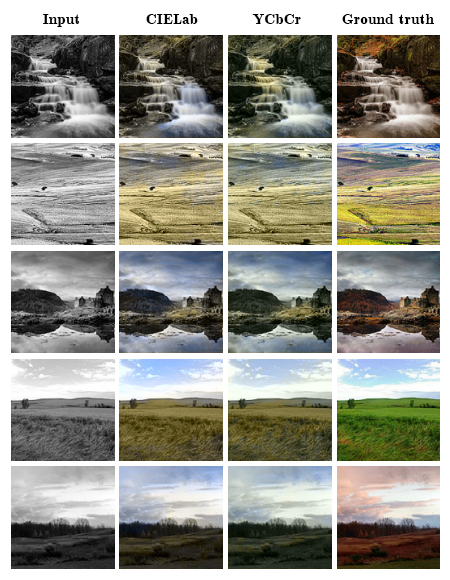
\includegraphics[width=0.6\textwidth]{YCbCr_vs_CIELab}
	\caption{YCbCr vs CIELab}
	\label{fig:YCbCr_vs_CIELab}
\end{figure}

\begin{figure}[h]
	\centering
	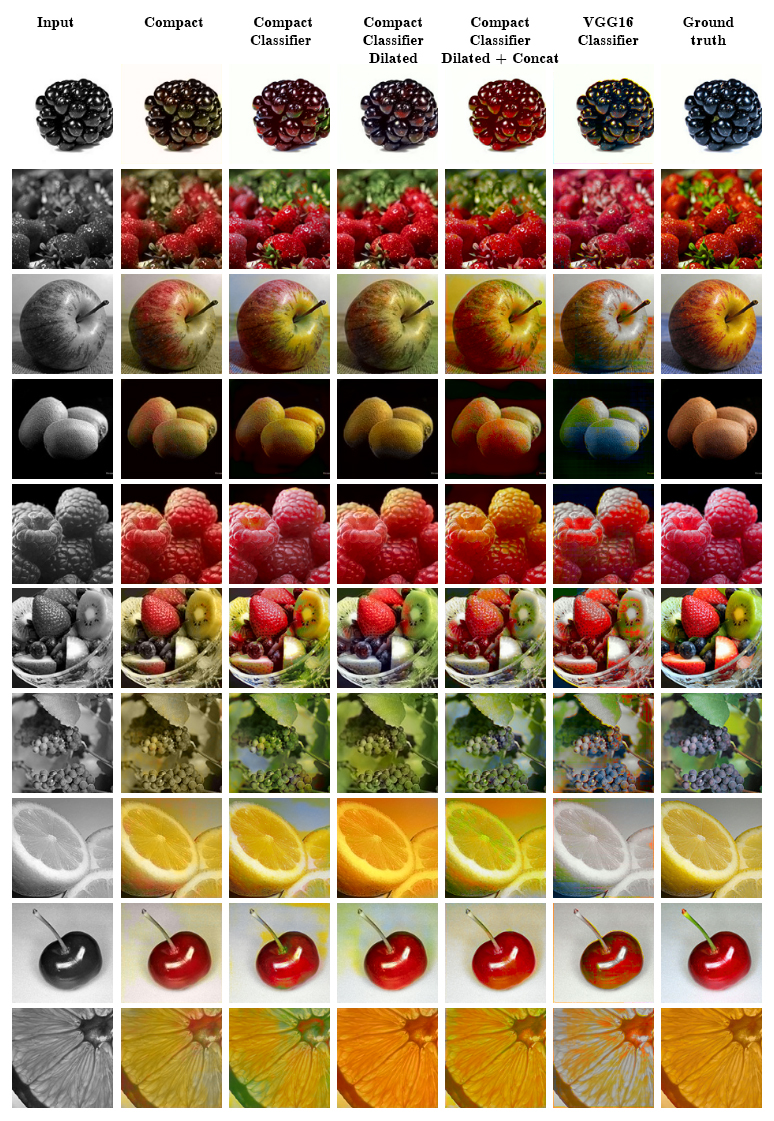
\includegraphics[width=0.9\textwidth]{set2}
	\caption{Results}
	\label{fig:results}
\end{figure}


